\documentclass[12pt]{article}
\usepackage[paperheight=11.5in,paperwidth=8.65in,margin=0in]{geometry}

% fontspec needs XeLaTeXe 
\usepackage{fontspec}
\setmainfont{Arial}  % use for backcover
\setmonofont{APL385}  
%\setmainfont[Color=000000,Scale=5]{Arial} % use for frontcover

\usepackage{graphicx}
\usepackage[dvipsnames]{xcolor}
\usepackage{colortbl}

\newcommand{\jodhspace}{\hspace{0.08\textwidth}}
\newcommand{\jodbackspace}{\hspace{0.04\textwidth}}
\newcommand{\jodcubewidth}{0.36}
\newcommand{\jodauthorwidth}{0.25}
\newcommand{\jodtxtwidth}{0.35}   % MAGIC NUMBERS: space + cube + txt < 1.0 & author < cube

\newcommand{\rowacolor}{\rowcolor{lightgray}}
\newcommand{\rowbcolor}{\rowcolor{lightgray}}
\newcommand{\rowccolor}{\rowcolor{lightgray}}

% cube colors used to build RGB cube
\newcommand{\jodred}[1]{\textcolor{red}{#1}}
\newcommand{\jodblue}[1]{\textcolor{RoyalBlue}{#1}}
\newcommand{\jodgreen}[1]{\textcolor{PineGreen}{#1}}
\newcommand{\jodcell}{\cellcolor{lightgray}}

\setlength\arrayrulewidth{6pt}\arrayrulecolor{lightgray}
\setlength\doublerulesep{6pt}\doublerulesepcolor{yellow}

\begin{document}

\thispagestyle{empty}

\jodbackspace
%\begin{tabular}{l >{\centering\arraybackslash}m{1in} l}
\begin{tabular}{ll}
\jodcell & \\
\jodcell & \\ 
%\jodcell & \\ 
\jodcell  & 
\begin{minipage}{\jodtxtwidth\textwidth}
\jodgreen{In 1991 I read a \texttt{USENET} message about a new
programming language called J. Kenneth Iverson, J's Turing 
award winning designer, was famous for his first language \textsl{APL}
so I knew J was worth a look. J did not disappoint. J's rare combination of theoretical 
coherence, productivity, array orientation and elegance is a daily delight.}

\smallskip

\jodgreen{JOD is a J programming tool. The inspiration for JOD comes 
from Roger Hui and Kenneth Iverson's \emph{Dictionary of J}: a seminal 
document that correctly highlights the power of the J word.} 

\begin{flushleft}
\jodgreen{\emph{John D. Baker}}\\
\jodgreen{\emph{April 2012}}\\
\jodgreen{\emph{St. Louis, Missouri}}
\end{flushleft}
\end{minipage}  \\
\jodcell & \\ 
\jodcell & \\
\jodcell 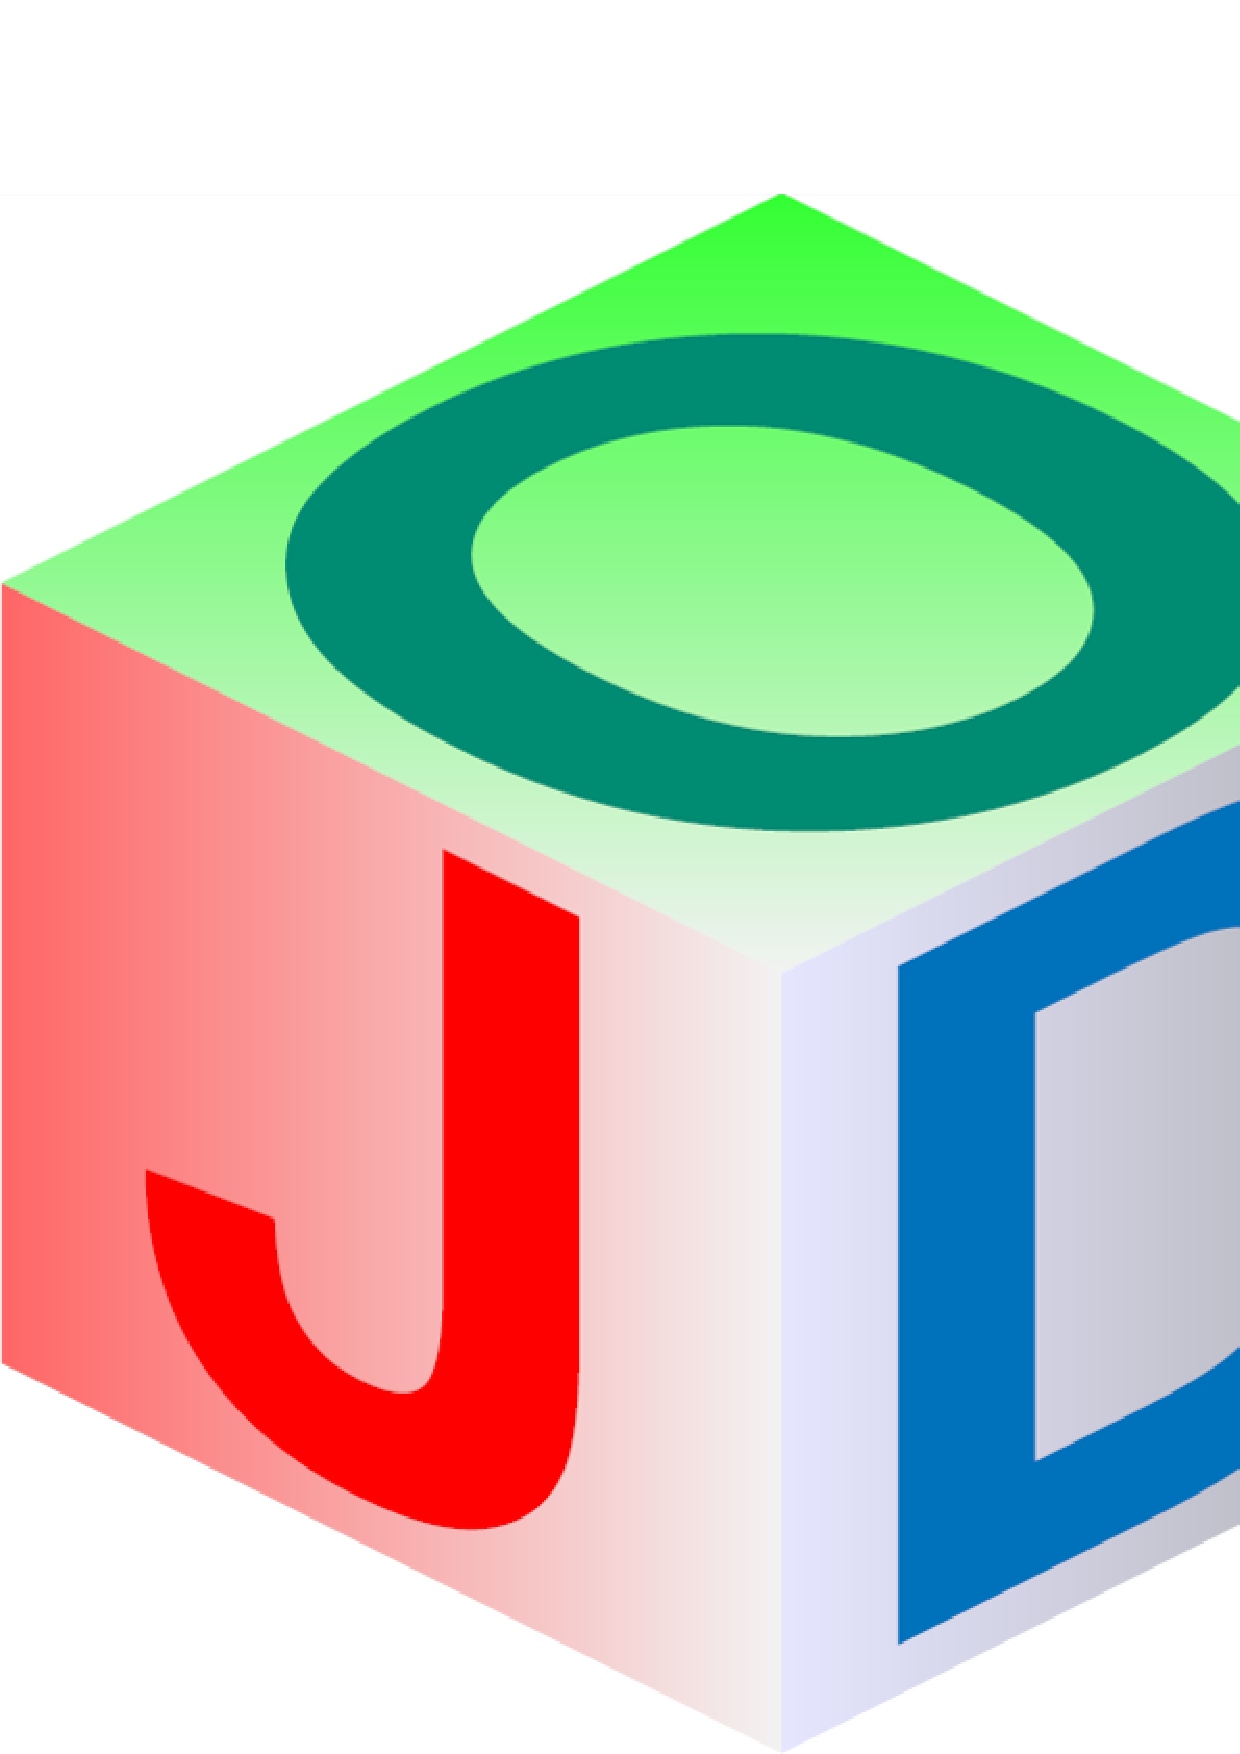
\includegraphics[width=\jodcubewidth\textwidth]{jodRGBcube.png} & \\
\jodcell & \\ 
\jodcell & \\
\jodcell 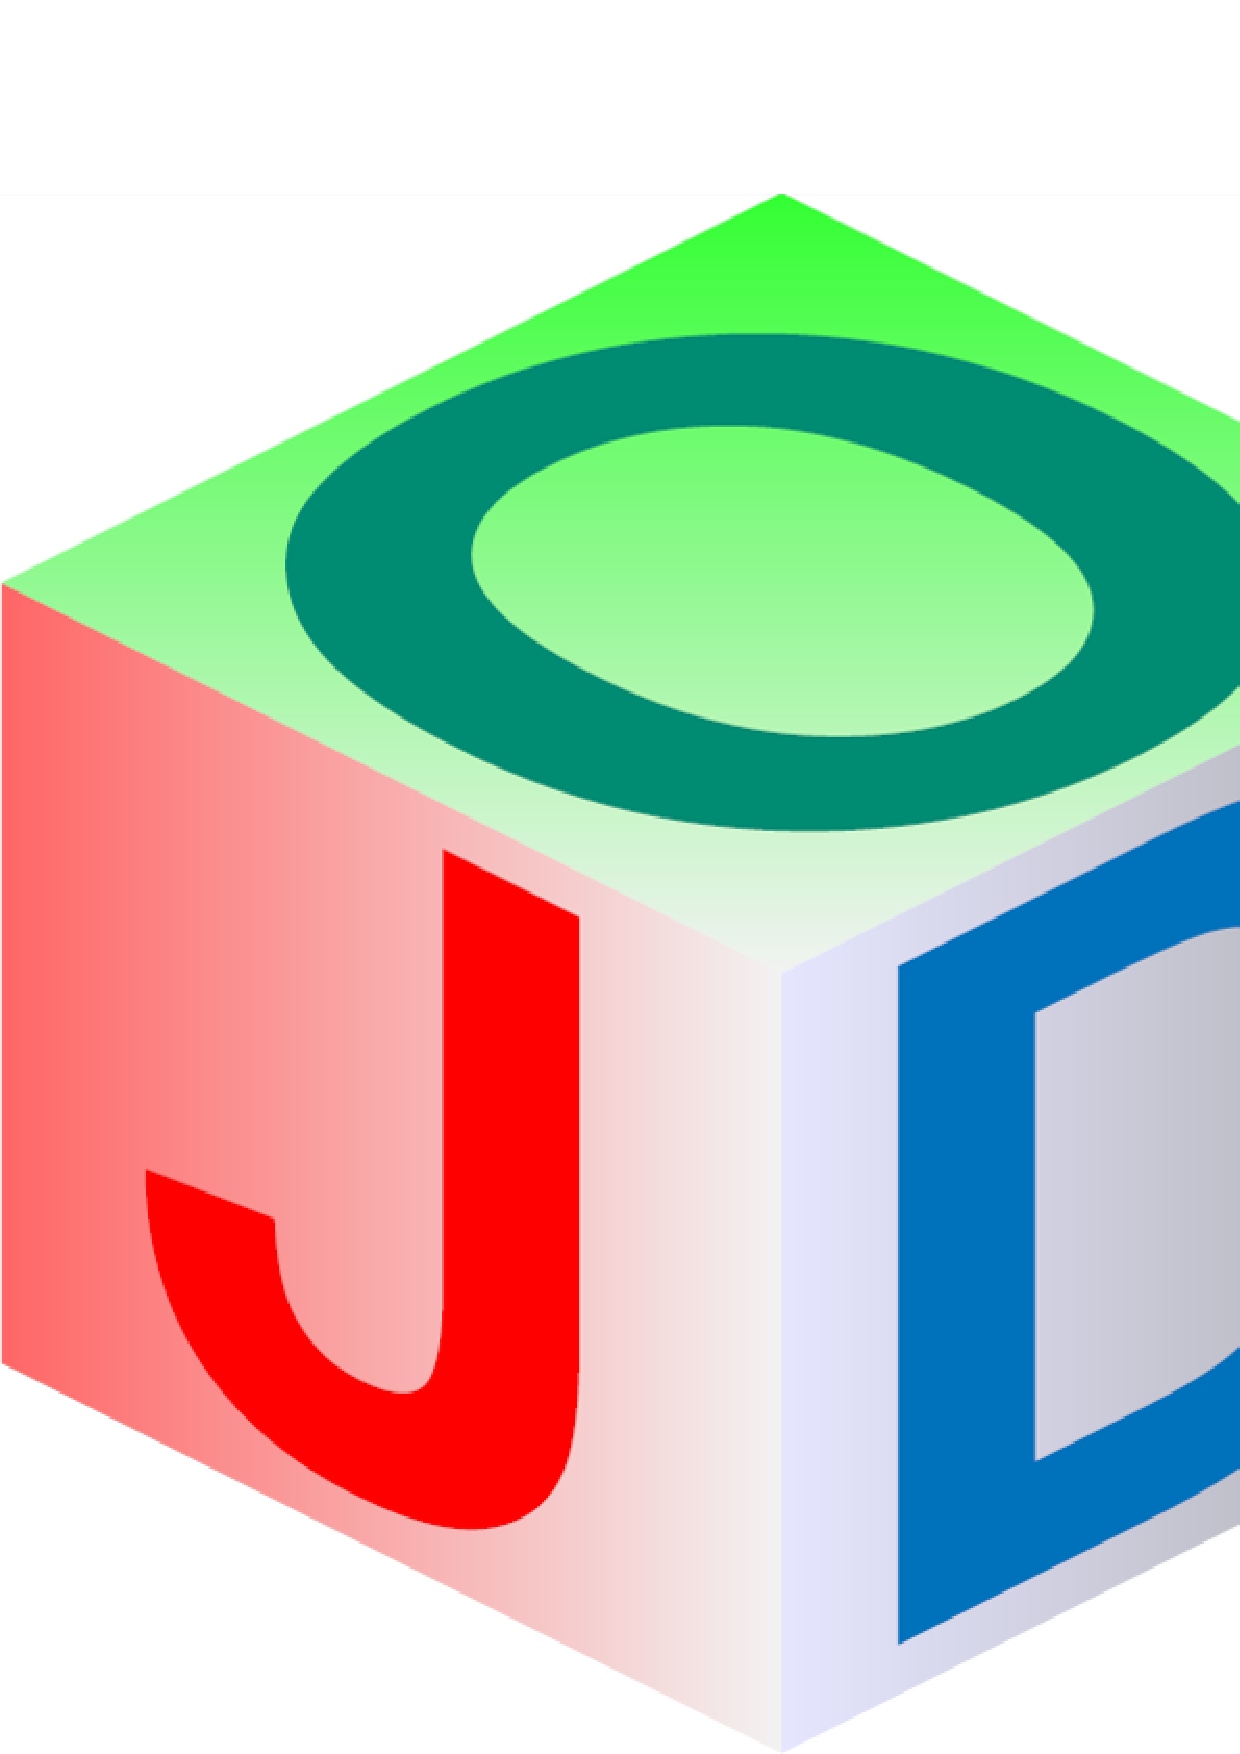
\includegraphics[width=\jodcubewidth\textwidth]{jodRGBcube.png} & \\ 
\jodcell & \\ 
\jodcell & \\ 
\jodcell & \\ 
\end{tabular}

\end{document}